
%%%%%%%%%%%%%%%%%%%%%%%%%%%%%%%%%%
\begin{frame} [plain]
    \frametitle{}
    \Background[1] 
    \begin{center}
    {\huge 第20讲:激光致冷技术}
    \end{center}  
    \addtocounter{framenumber}{-1}   
\end{frame}

\begin{frame} 
\frametitle{引入}
  \begin{center}
       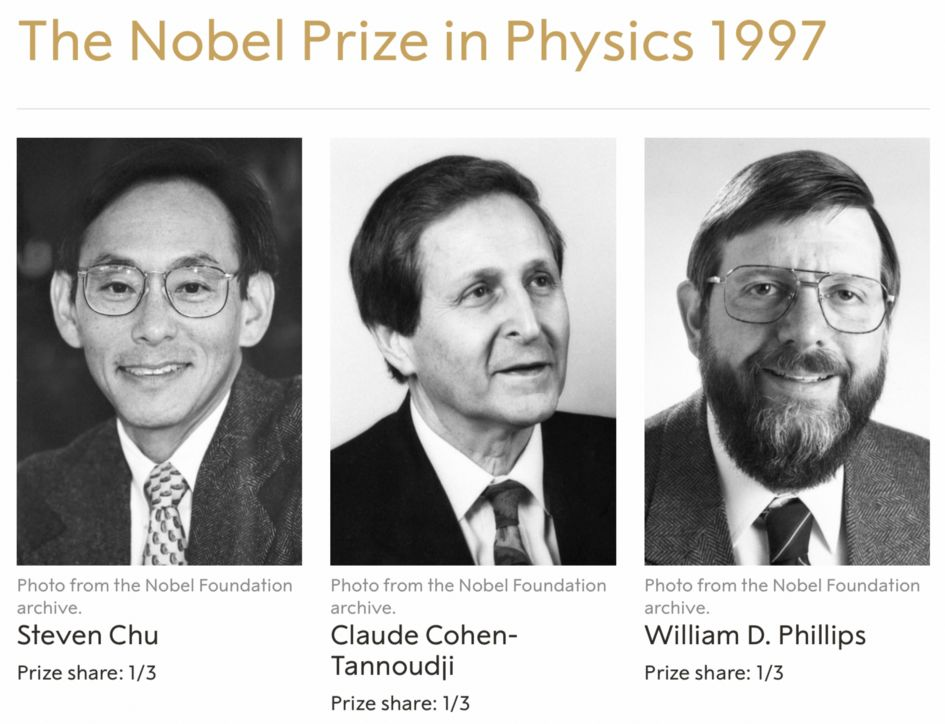
\includegraphics[width=0.48\textwidth]{figs/2022-05-27-23-18-37.png}
  \end{center}
低温的重要性: 
\begin{itemize}
    \item 玻色-爱因斯坦凝聚, 超导, 超流, 量子计算, 量子通信, 高精度原子钟, 精密测量, 量子模拟, ...
\end{itemize}
\end{frame}

\section{1. 温度-能量关系}

\begin{frame} 
\frametitle{能量均分定理}
对于近独立粒子体系,设每个粒子的自由度为N, 则体系的总能量为
\[ E=E_k= \frac{N}{2} k_B T\]
即, 每个自由度分得的动能为 $\frac{1}{2} k_B T$ \\ {\vspace*{1.3em}}

对于三维理想气体
\[ \frac{1}{2} m v_x ^2 = \frac{1}{2} k_B T\]
速度与温度的关系
\[ v_x = \frac{\sqrt{k_B T}}{m}, \quad v = \frac{\sqrt{3 k_B T}}{m} \]
\end{frame}

\begin{frame} 
\frametitle{}
 动量与温度的关系 
 \[ p=mv =\sqrt{3 k_B T}\]
 动能与温度的关系 
 \[E_k=\frac{p^2}{2m} = \frac{3 k_B T}{2m}\]
\end{frame}

\section{2. 多普勒冷却}

\begin{frame} 
\frametitle{}
\begin{columns}
    \begin{column}[t]{0.72\linewidth}
     要点:
     \begin{itemize}
         \item 原子迎着激光束运动时, 接受到蓝移激光,
         \item 如果激光的频率稍低于原子的共振吸收频率 (红失谐), 则只有在原子迎着激光束运动时才收吸光子,
         \item 原子吸收光子能量的同时, 也获得光子动量, 导致原子的速度变慢,
         \item 自发发射方向的随机性,导致原子因发射光子而获得速度的时间平均为零,
         \item 多次多普勒效应导致原子冷却, 
         \item 光子辐射的反冲动量是冷却极限.
     \end{itemize}
    \end{column}
    \begin{column}[t]{0.28\linewidth} 
       \begin{center}
            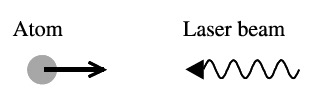
\includegraphics[width=1.0\textwidth]{figs/2022-05-30-12-11-01.png}
       \end{center}
    \end{column}
\end{columns} 
\end{frame}

\begin{frame} 
\frametitle{}
* 从能量角度看, 原子吸收红失谐光子, 发射零失谐光子, 发射的能量大于吸收的能量,每个过程都在损失能量 \\ 
设原子的共振频率为$ \omega $,  激光的频率为 $ \omega_0 $, 失谐为 $ \delta=\omega-\omega_0 $, 则每一个吸收发射过程损失的能量:
\[ \varepsilon = \hbar \delta \]
设初始原子温度为T, 对应的动能为 $E_k=\frac{p^2}{2m}$, 动能完全损失时, 有:
\[ N_{stop}= \frac{E_k}{\varepsilon} = \frac{p^2}{2m \varepsilon}= \frac{ 3 k_B T }{2m\hbar (\omega-\omega_0) } \]
反冲动能(冷却极限): 
\[ E_{min} = \hbar \omega_0=\frac{3 k_B T_{min}}{2m}\]
\[ T_{min} = \frac{2 m \hbar \omega_0}{3 k_B} \]
\end{frame}

\begin{frame} 
\frametitle{光学黏团与磁光原子阱}
\begin{columns}
    \begin{column}[t]{0.76\linewidth}
        两个电流方向反向的线圈产生的磁场
        \[  \mathbf{B} = B_0 (x \mathbf{e}_x + y \mathbf{e}_y -2z \mathbf{e}_z)\]
        磁场大小
        \[ B= B_0  (x^2 + y^2 + 4z^2)\]
        * 坐标原点处磁场取最小值(零) \\ 
        原子的塞曼能 
        \[ E_{zm} = g_J \mu_B B M_J \]
        *$M_J > 0 $时,弱场搜寻态: 磁四极表现为吸力, 把原子捕获在B最小处 (塞曼能最小), \\  
        $M_J < 0 $时,强场搜寻态: 磁四极表现为拆力, 把原子推向B最小处 \\ 
    \end{column}
    \begin{column}[t]{0.230\linewidth} 
       \begin{center}
            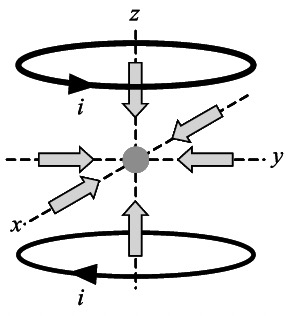
\includegraphics[width=1.0\textwidth]{figs/2022-05-30-12-43-21.png}
            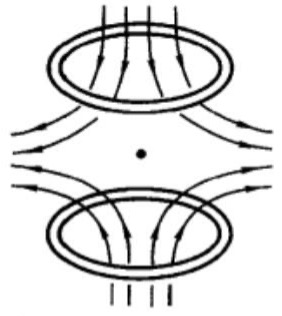
\includegraphics[width=1.0\textwidth]{figs/2022-05-30-13-11-59.png}
       \end{center}
    \end{column}
\end{columns}   
\end{frame}

\section{3. 偏振梯度冷却}

\begin{frame} 
    \frametitle{偏振梯度冷却}
    \begin{columns}
        \begin{column}[t]{0.6\linewidth}
            原子的量子数
            \[ \begin{aligned}
                n & = 1, 2 , \cdots\\
                l & = 0, 1, 2, \cdots, n-1; \quad  s= 1/2 \\
                m_l & = 0, \pm 1 , \pm 2, \pm l, ; \quad  m_s= \pm 1/2 
            \end{aligned}\] 
            二能级原子的总角动量与总磁量子数 
            \[ \begin{aligned}
                \rs{1}: &J=1/2  \quad \quad \,\,\, \rs{2}: J=3/2 \\
                \rs{1}: &M_J=\pm 1/2 \quad \rs{2}: M_J =\pm 1/2,\pm 3/2
            \end{aligned}\] 
        \end{column}
        \begin{column}[t]{0.4\linewidth} 
           \begin{center}
                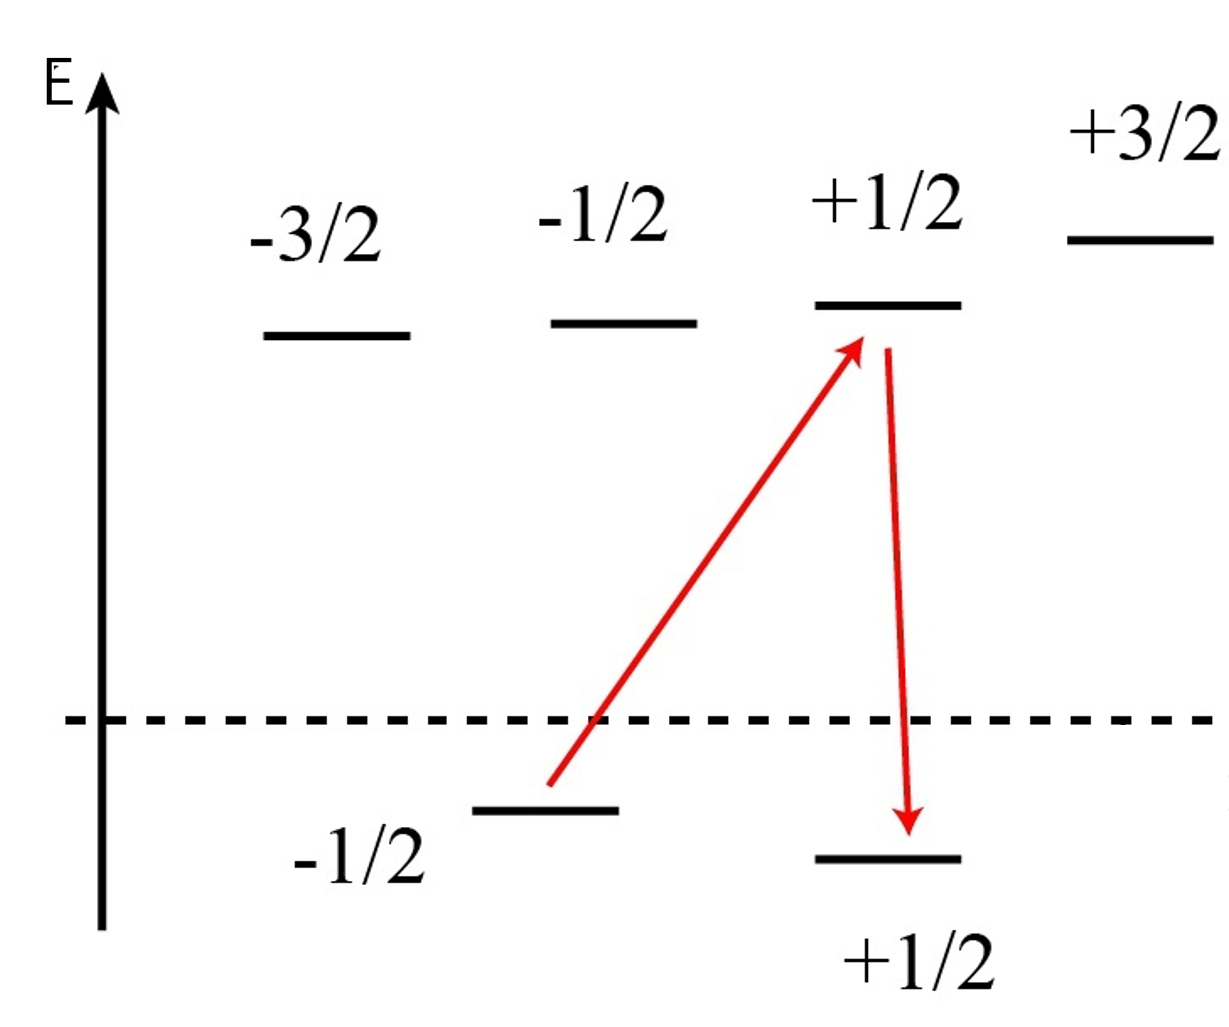
\includegraphics[width=1.0\textwidth]{figs/30.png}
           \end{center}
        \end{column}
    \end{columns}   
    \end{frame}

    \begin{frame} 
    \frametitle{}
    \begin{columns}
    \begin{column}[t]{0.65\linewidth}
    ~\\
    激光腔场是两偏振波构成的驻波. \\ {\vspace*{0.3em}}
    {\Bullet}在红失谐条件下\\ 
    (1) 在位点(2)只有$M_J=-1/2$的$\rs{1}$原子吸收光子(更接近共振吸收),并激发到$M_J=+1/2$的$\rs{2}$ (光子的自旋量子数为$1$)  \\ 
    (2) 而在位点(4)只有$M_J=1/2$的$\rs{1}$原子吸收光子并激发到$M_J=+3/2$的$\rs{2}$   \\ {\vspace*{0.3em}}
    {\Bullet} $\rs{2}$ 原子自发发射, 满足选择定则 ($\Delta M_J = 0, \pm 1)$的都可能发生, 并以更大概率跃迁到能量更低的自旋态, 比如(1)(5)处的 $M_J=+1/2$的$\rs{1}$, (3) 处的 $M_J=-1/2$的$\rs{1}$ \\ {\vspace*{0.3em}}
    {\Bullet} 大概率过程: $1\to2\to3\to4\to5\to \cdots$,  每次吸收-发射, 原子损失部分能量,被冷却.
    \end{column}
    \begin{column}[t]{0.35\linewidth} 
        \begin{center}
            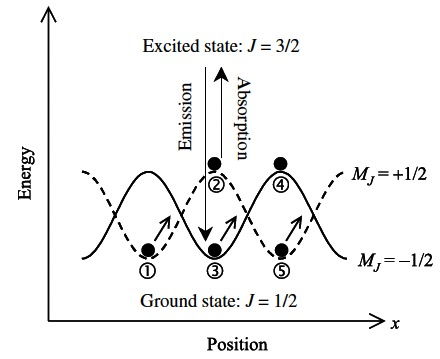
\includegraphics[width=1.0\textwidth]{figs/2022-05-30-14-49-27.png}
        \end{center}
    \end{column}
    \end{columns}
    \end{frame}

    \section{4. 拉曼冷却}

    \begin{frame} 
    \frametitle{}
    拉曼跃迁为双光子过程,如图所示
      \begin{center}
           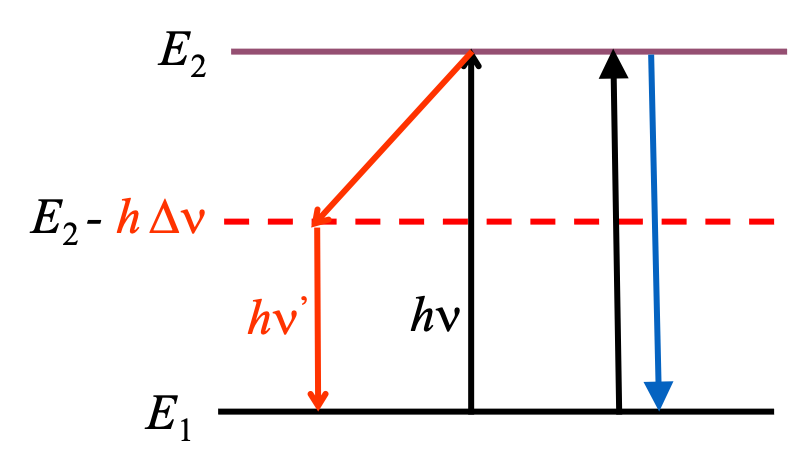
\includegraphics[width=0.4\textwidth]{figs/31.png}
      \end{center}
    采用能带调控技术在 $\rs{1}$ 和 $\rs{2}$  插入一个亚稳态 $\rs{i} $, 并满足选择定则如图选择定则的要求.  \\ {\vspace*{2.3em}} 
    特点: 可以得到更低的温度 \\ 
    原来的光子反冲能量$h \nu $, 现在的反冲能量$h \nu' = h \nu - h \Delta \nu $, 低温量级 $\mu K$
    \end{frame}

    \section{5. 蒸发冷却}

    \begin{frame} 
    \frametitle{}
    \begin{columns}
        \begin{column}[t]{0.58\linewidth}
    技术要点:
    \begin{itemize}
        \item 前面的技术都基于理想气体模型, 是不考虑原子之间的相互作用的.
        \item 若把已达到技术极限的冷原子放在一起, 则必须考虑原子间的相互作用. 
        \item 红外蒸发技术可以把能量较高的原子从腔内去除.
        \item 蒸发原子可以极大降低余下原子的温度.
        \item 低温量级 $nK$
    \end{itemize}
    \end{column}
    \begin{column}[t]{0.42\linewidth} 
        \begin{center}
            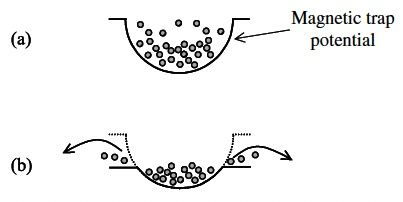
\includegraphics[width=1.0\textwidth]{figs/2022-05-30-16-50-58.png}
        \end{center}
    \end{column}
    \end{columns}   
    \end{frame}

    
    \begin{frame} 
    \frametitle{}
    ~\\
    基于激光冷却技术,目前已实现多种物质的玻色-爱因斯坦凝聚态, 是继气、液、固以及等离子态之后物质的第五凝聚态. 
\[
    \begin{array}{lll}
        \hline \text { Atom } & \text { Isotope } & \begin{array}{l}
        \text { Year of } \\
        \text { observation }
        \end{array} \\
        \hline \text { Rubidium } & { }^{87} \mathrm{Rb} & 1995 \\
        \text { Sodium } & { }^{23} \mathrm{Na} & 1995 \\
        \text { Lithium } & { }^{7} \mathrm{Li} & 1997 \\
        \text { Hydrogen } & { }^{1} \mathrm{H} & 1998 \\
        \text { Rubidium } & { }^{85} \mathrm{Rb} & 2000 \\
        \text { Helium } & { }^{4} \mathrm{He} & 2001 \\
        \text { Potassium } & { }^{41} \mathrm{~K} & 2001 \\
        \text { Cesium } & { }^{133} \mathrm{Cs} & 2002 \\
        \text { Ytterbium } & { }^{174} \mathrm{Yb} & 2003 \\
        \hline
        \end{array}    
\]
    \end{frame}

    \begin{frame} 
    \frametitle{}
    \[
        \begin{array}{lll}
            \hline \text { Atom } & \text { Isotope } & \begin{array}{l}
            \text { Year of } \\
            \text { observation }
            \end{array} \\
            \hline 
            \text { Chromium } & { }^{52} \mathrm{Cr} & 2005 \\
            \text {polaritons} &  & (Kasprzak 2006) \\ 
            \text {magnon} &  & (Demokritov 2006) \\ 
            \text {calcium} & & (Kraft 2009) \\ 
            \text {strontium} & & (Stellmer 2010) \\ 
            \text {photons} & & (Klaers 2010) \\ 
            \text {excitons} & & (Dai 2011) \\
            \hline
            \end{array}  
    \]
    \end{frame}

    \begin{frame} 
    \frametitle{}
    玻色-爱因斯坦凝聚态, 目前最直接的应用是只有一个原子作为增益介质的冷原子激光器(单原子激光),直接得到非经典光场
      \begin{center}
           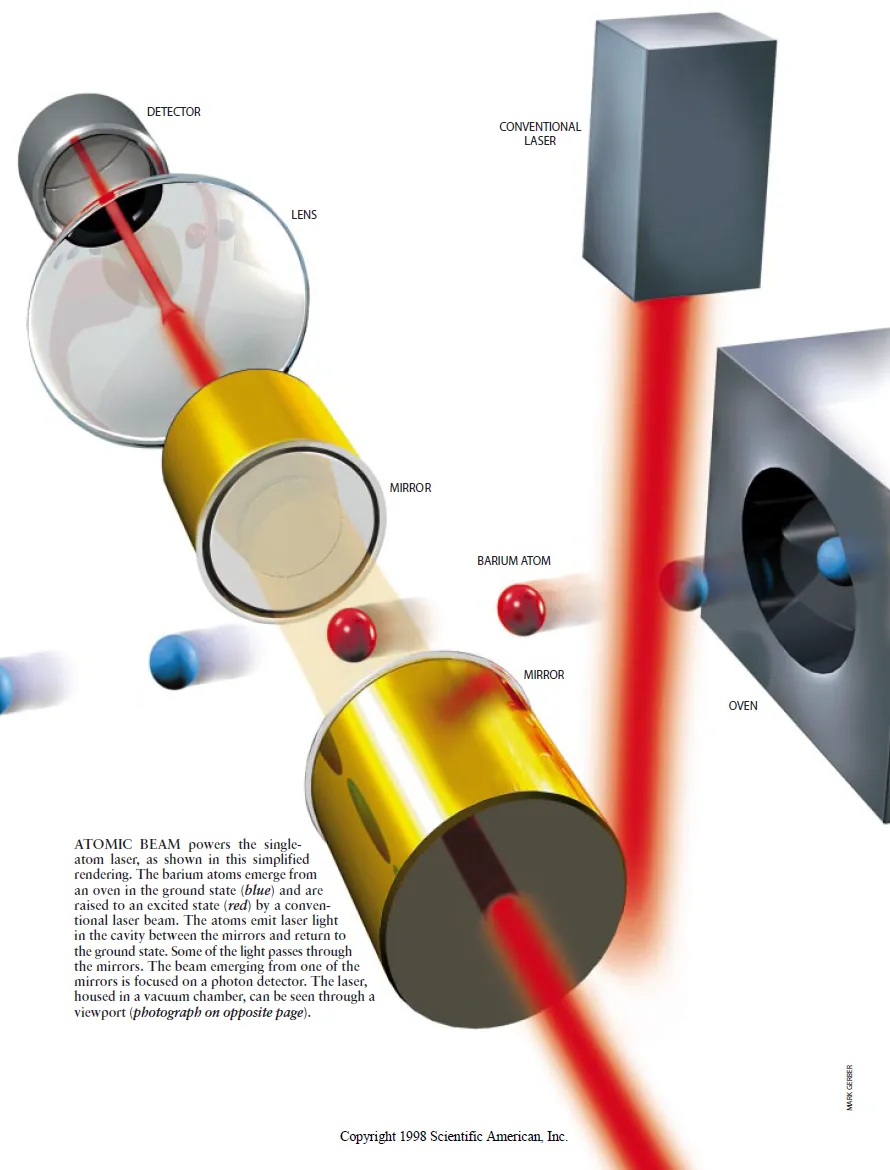
\includegraphics[width=0.4\textwidth]{figs/2022-05-30-17-08-39.png}
      \end{center}
    \end{frame}

    \section{6. 原子在光场中的运动}

    \begin{frame} 
    \frametitle{哈密顿}
    静态原子-光场体系的哈密顿: 
    \[\begin{aligned}
        H &= \hbar \omega S_z + \hbar \omega_0 (a^{\dagger}  a +\frac{1}{2}) + \hbar g ( a S^- + S^+ a ^{\dagger}) 
    \end{aligned} \] 
    当考虑原子的运动时,得增强动能项, 并考虑光场的偏振.
    \[\begin{aligned}
        H &= \hbar \omega S_z + \frac{|p|^2}{2m} + \sum _{\sigma=1} ^2 \hbar \omega_0 (a^{\dagger}_\sigma  a_\sigma +\frac{1}{2}) + \frac{1}{2} i \hbar g \sum _{\sigma=1} ^2 ( S^+ a ^{\dagger} _\sigma e^{i k_i x} + a_\sigma S^- e^{-i k_i x} )  \cdots (1)
    \end{aligned} \] 
    \end{frame}

    \begin{frame} 
    \frametitle{波函数}
        设原子的基态是初态$\rs{1}$, 动量为$\vec{p}_0$, 可写成 
        \[\rs{1,\vec{p}_0}\]
        光场初态, 左偏光 $\rs{n_1}$, 右偏光 $\rs{n_2}$, 可写成
        \[ \rs{n_1} \rs{n_2}\]
        因此, 体系的初态函数:
        \[\rs{\Psi_0} = \rs{n_1} \rs{n_2}\rs{1,\vec{p}_0}\]
    \end{frame}

    \begin{frame} 
    \frametitle{}
         原子进入光场. \\  
         吸收一个左偏光子的激发态:
         \[ \rs{\Psi_1}= \rs{n_1 -1} \rs{n_2}\rs{2,\vec{p}_0+ \hbar \vec{k}_1}\]
         吸收一个右偏光子的激发态:
         \[ \rs{\Psi_2}= \rs{n_1 } \rs{n_2 -1}\rs{2,\vec{p}_0+ \hbar \vec{k}_2}\]
    \end{frame}

    \begin{frame} 
    \frametitle{}
         考虑强耦合情况, 即只考虑受激发射. \\ 
         (1) 设体系处于激发态 $\rs{\Psi_1}$,  \\ 
         \begin{itemize}
             \item 若受激发射一个左偏光子, 则态函数回到 
             \[\rs{\Psi_0} = \rs{n_1} \rs{n_2}\rs{1,\vec{p}_0}\]
             \item 若受激发射一个右偏光子, 则态函数变为
             \[\rs{\Psi_3}= \rs{n_1 -1} \rs{n_2 +1 }\rs{1,\vec{p}_0+ \hbar \vec{k}_1 - \hbar \vec{k}_2}\]
         \end{itemize}
         (2) 设体系处于激发态 $\rs{\Psi_2}$,  \\ 
         \begin{itemize}
             \item 若受激发射一个左偏光子, 则态函数变为
             \[\rs{\Psi_4}= \rs{n_1 +1} \rs{n_2 -1 }\rs{1,\vec{p}_0+ \hbar \vec{k}_2 - \hbar \vec{k}_1}\]
             \item 若受激发射一个右偏光子, 则态函数变回到
             \[\rs{\Psi_0} = \rs{n_1} \rs{n_2}\rs{1,\vec{p}_0}\]
         \end{itemize}
    \end{frame}

    \begin{frame} 
    \frametitle{}
        经过 $n$ 次吸收-发射后, 体系的波函数应该是:
        \[ \begin{cases}
            \rs{\Psi_n} = &\rs{n_1 - \frac{n}{2}} \rs{n_2 + \frac{n}{2} }\rs{1,\vec{p}_0 + \frac{n}{2} \hbar \vec{k}_1 - \frac{n}{2}\hbar \vec{k}_2} \quad (\text{when ~ n is even}) \\ 
            ~\\ 
            \rs{\Psi_n} = &\rs{n_1 - \frac{n+1}{2}} \rs{n_2 + \frac{n-1}{2} }\\ 
            & \otimes \rs{2,\vec{p}_0 + \frac{n+1}{2} \hbar \vec{k}_1 - \frac{n-1}{2}\hbar \vec{k}_2} \quad (\text{when ~ n is odd}) 
        \end{cases} \]
        ~ \\ 
        $\{\rs{\Psi_n}\}$构成无相互作用体系的正交归一完全集.  \\ 
        有相互作用体系的波函数可以在这个完全集上展开 
        \[ \rs{\Psi_n (t)}  =  \int d \vec{p} c_n(\vec{p},t) \rs{\Psi_n} \qquad \cdots (2)\]
    \end{frame}

    \begin{frame} 
    \frametitle{薛定谔方程}
        把(1)式的哈密顿和(2)的波函数,代入含时薛定谔方程
        \[ i \hbar \frac{\partial \psi}{\partial t} = H \psi \]
        得到有关展开系数的方程 ($even$)
        \[ \begin{aligned}
            i \hbar \frac{d  }{d t} c_n = & \left\{ \left( n_1 - \frac{n}{2} \right) \hbar \omega_0  + \left( n_2 + \frac{n}{2} \right) \hbar \omega_0  \right.\\ 
            & + \left. \frac{1}{2m} \left(\vec{p}_0 +\frac{n}{2} \hbar \vec{k}_1 - \frac{n}{2}\hbar \vec{k}_2\right)^2 -  \frac{n}{2} \hbar \omega \right\} c_n \\
            & + i \frac{g}{2} \hbar \left( \sqrt{n_1 - \frac{n}{2}} c_{n-1} -\sqrt{n_2 + \frac{n}{2}} c_{n+1}
            \right)
        \end{aligned}\] 
    \end{frame}

    \begin{frame} 
    \frametitle{}
         作用记号
         \[ E_N = \left( n_1 + n_2 -\frac{1}{2} \right) \hbar \omega_0 + \frac{1}{2m} (p^2 _x + p^2 _y)\]
         及演化形式
         \[C_n = c_n e ^{iE_N t}\]
         方程可简化为
         \[ \begin{aligned}
            i  \frac{d  }{d t} C_n &= \frac{1}{2} \Delta C_n + \left[ \frac{n^2 \hbar }{8m} ( \vec{k}_1 - \vec{k}_2)^2  + \frac{n \vec{p}_0 ^2 }{2m} ( \vec{k}_1 - \vec{k}_2)^2 
            \right] C_n\\
            & + i \frac{g}{2} \hbar \left( \sqrt{n_1 - \frac{n}{2}} C_{n-1} -\sqrt{n_2 + \frac{n}{2}} C_{n+1}
            \right)  \\
         \end{aligned}\] 
         式中 $\Delta = \omega_0 - \omega$, 是失谐频率.
    \end{frame}

    \begin{frame} 
    \frametitle{}
         同理, 得 ($odd$) 
         \[ \begin{aligned}
            i  \frac{d  }{d t} C_n &= - \frac{1}{2} \Delta C_n + \left\{ \frac{\hbar }{8m} [(n+1) \vec{k}_1 - (n-1)\vec{k}_2]^2 \right. \\ 
            & \left. + \frac{\vec{p}_0 ^2 }{2m} [ (n+1) \vec{k}_1 - (n-1) \vec{k}_2]  
            \right\} C_n\\
            & + i \frac{g}{2} \hbar \left( \sqrt{n_1 - \frac{n-1}{2}} C_{n-1} -\sqrt{n_2 + \frac{n+1}{2}} C_{n+1}
            \right)  \\
         \end{aligned}\] 
    \end{frame}

    \begin{frame} 
    \frametitle{}
         考虑到光场的光子数远远大于事件数
         \[ n_1, n_2 \gg n \]
         有: 
         \[ \sqrt{n_\sigma \pm  \frac{n}{2}}  \approx \sqrt{n_\sigma \pm  \frac{n\pm 1}{2}} \approx  \sqrt{n_\sigma} = \sqrt{\bar{n}_\sigma} = \sqrt{N}\]
         方程可进一步简化为:
    \end{frame}
    
    \begin{frame} 
    \frametitle{}
             
            \[ \begin{cases}
                \frac{d  }{d t} C_n &= - i \left[ \frac{1}{2} \Delta + b (n^2 +2nq)  \right] C_n + \frac{1}{2} \Omega (C_{n-1} - C_{n+1})  \quad (\text{even})\\ 
                ~\\
                \frac{d  }{d t} C_n &= - i \left[ - \frac{1}{2} \Delta + b (n^2 +2nq)  \right] C_n + \frac{1}{2} \Omega (C_{n-1} - C_{n+1}) \quad (\text{odd}) \\  
            \end{cases} \]
    上式,定义如下记号
    \[ \Omega = g \sqrt{N}, \quad \hbar b = \frac{\hbar ^2 k^2}{2m}, \quad q = \frac{p_x}{\hbar k} \]
    \end{frame}

    \begin{frame} 
    \frametitle{求解}
    考虑原子共振与光场共振 $\Delta = \omega_0 - \omega =0$ \\ 
         (1) 若原子的动量沿光场传播方向的投影为零,$p_x =0$ \\ 
        无论奇偶, 方程化为:
        \[ \frac{d  }{d t} C_n = \frac{1}{2} \Omega (C_{n-1} - C_{n+1})\]
        令 $s= \Omega t$
        方程化为
        \[ 2\frac{d  }{d t} C_n(s) = \frac{1}{2} (C_{n-1} - C_{n+1})\]
        这是Bessel函数的递推式, 因此方程的解为
        \[C_n(t) = J_n (\Omega t)\]
    \end{frame}

    \begin{frame} 
    \frametitle{}
        体系处于态 \[\rs{\Psi_n} = \rs{n_1 - \frac{n}{2}} \rs{n_2 + \frac{n}{2} }\rs{1,\vec{p}_0 + \frac{n}{2} \hbar \vec{k}_1 - \frac{n}{2}\hbar \vec{k}_2} \]
        的概率为:
        \[ P_n(t) = |C_n(t)|^2 = J_n ^2 (\Omega t) \]
        对应的动量增量为:
        \[ \vec{p} =  \frac{n}{2} \hbar (\vec{k}_1- \vec{k}_2)\]
    \end{frame}

    \begin{frame} 
    \frametitle{}
    考虑原子共振与光场共振 $\Delta = \omega_0 - \omega =0$ \\ 
    (2) 若原子的动量沿光场传播方向的投影为零,$p_x \not =0$ \\ 
    无论奇偶, 方程化为:
    \[ \frac{d  }{d t} C_n =  - i b n^2 -i 2(n b q )C_n + \frac{1}{2} \Omega (C_{n-1} - C_{n+1})\]
    不考虑发射光子带来的反冲能量项 $- i b n^2$, 
    \[ \frac{d  }{d t} C_n =  -i 2(n b q) C_n + \frac{1}{2} \Omega (C_{n-1} - C_{n+1})\]
    令\[ C_N= C_n e^{i(nbq)t}\]
    \end{frame}

    \begin{frame} 
    \frametitle{}
        方程变为
        \[ 2\frac{d  }{d t} C_N = -i \frac{bq}{\Omega \cos (bqt) } \left[2n C_N - \frac{\Omega}{bq} \sin (bqt) (C_{n-1} + C_{n+1})\right]\]
        解为:
        \[C_N (t) = J_n (\frac{\Omega}{bq} \sin (bqt)) \]
        处于 $\rs{\Psi_n}$态的概率为
        \[P_n(t) = |C_N (t)|^2 = J^2 _n (\frac{\Omega}{bq} \sin (bqt))\]
        呈现出频率为$bq=\frac{p_x k}{2m} $的振荡行为.
    \end{frame}

    \begin{frame}
        \frametitle{课程小结}
        \begin{itemize}
            \item 光场量子化~ 量子谐振子 ~ 真空态 ~ 数态 ~ 产生湮灭算符 ~ 场算符 ~ 正交分量算符 ~ 相位算符 ~ 相图  
            \item 相干态 ~ 压缩态 ~ 辐射场  
            \item 光子计数 ~~ 关联函数~~反聚束
            \item 光场表象
            \item 光与原子相互作用
            \item 光腔中的原子
        \end{itemize}     
    \end{frame}